% Autor: Francisco Javier Barranco Tena
% Apendice con los resultados de los experimentos realizados en el desarrollo del TFG
% Alt + z o Option + z para activar el word wrap en Visual Studio Code

\section{Experimento 1: Entrenamiento con datos de Estados Unidos y validación cruzada}
En la figura \ref{fig:exp1_val_output} se pueden ver los resultados de la validación de los modelos en cada iteración del experimento 1. En la sección \ref{SEC:EXP1} se ha explicado en detalle cómo se ha llevado a cabo este experimento y se han mostrado un resumen de los resultados obtenidos en cada iteración. En la tabla \ref{tab:exp1_results} se pueden ver estos resultados.

% Añadimos ../img/exp1-val-output.png
\begin{figure}[H]
    \centering
    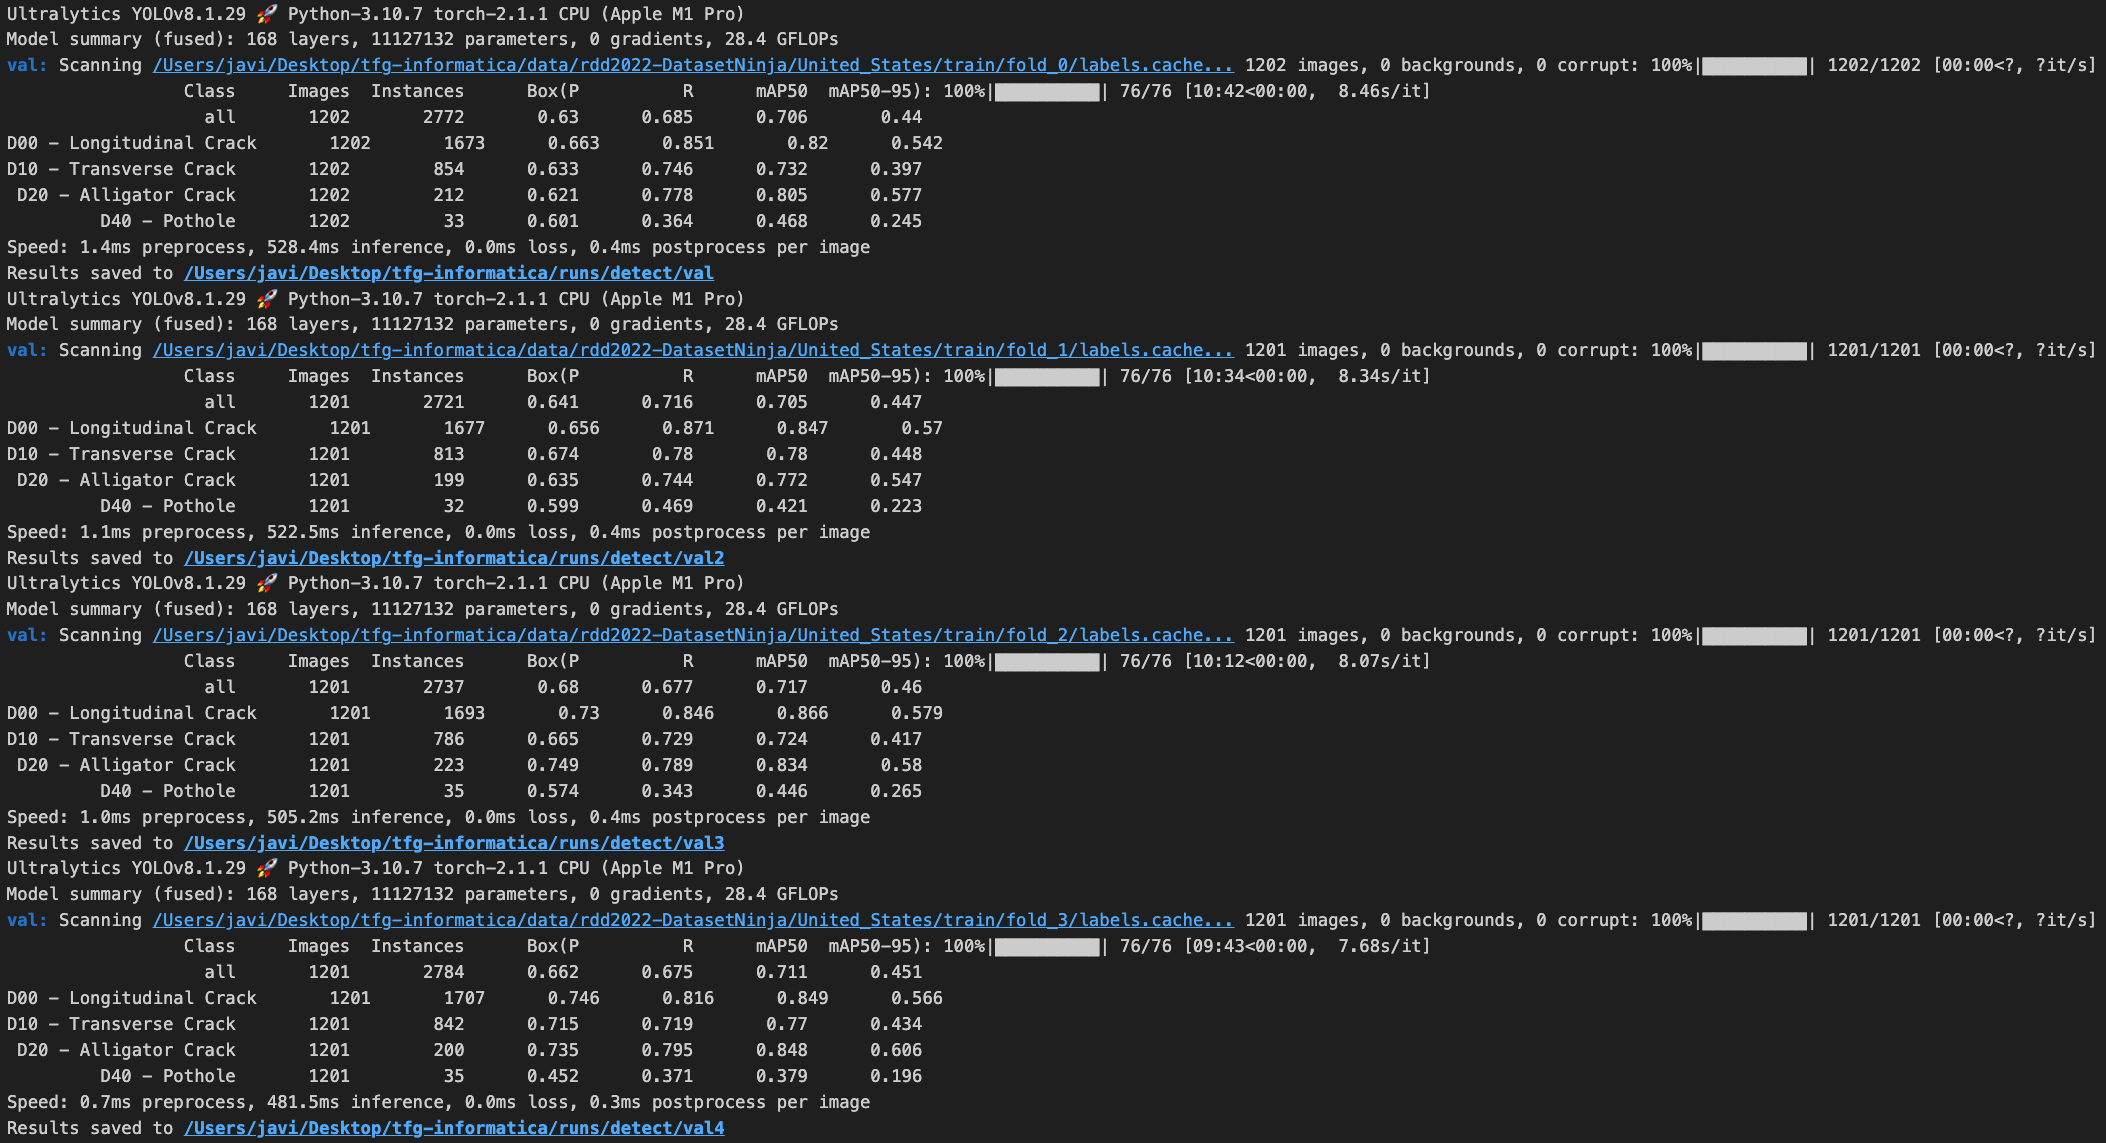
\includegraphics[width=\textwidth,height=\textheight,keepaspectratio]{../img/exp1-val-output.png}
    \caption{Resultados de la validación de los modelos en cada iteración del experimento 1.}
    \label{fig:exp1_val_output}
\end{figure}